% ===========================================================================
% CORPO - Geracao de Dados - Limiar v1
% ===========================================================================

\begin{center}
{\large\bfseries Universidade Federal de Alagoas}\\[2pt]
{ECOM060 --- Instrumentação Eletrônica --- 2026.2}\\[10pt]
{\LARGE\bfseries Geração de Dados Brutos --- Limiar}\\[4pt]
{\large Característica Estática (Seção 3.3): Protocolo de Pequenos Incrementos Crescentes ---
Gerador Síncrono (\emph{Swing Equation})}\\[6pt]
{\normalsize Versão 1}
\end{center}

\vspace{4pt}
\noindent\textbf{Professor responsável:} Prof.\ Maurício Beltrão Rossiter\\
\textbf{Sistema atribuído:} Sistema 7 --- Gerador síncrono (\emph{swing equation})\\
\textbf{Rodada:} Orientação --- Geração de dados, Características estáticas (Seção 3.3)\\
\textbf{Tópico do Grupo 08:} Limiar\\
\textbf{Data:} 03 / 09 / 2026

\subsection*{Identificação da equipe}
\begin{center}
\begin{tabular}{ll}
\toprule
\textbf{Nome completo} & \textbf{Matrícula}\\
\midrule
Cleiber de Meireles da Silva Junnior & 20113298\\
Leonardo Lima Barbosa Pereira & 22110875\\
Willian Tcheldon Oliveira Santos & 17212878\\
\bottomrule
\end{tabular}
\end{center}

% ===========================================================================
\section{Contexto}

Este relatório documenta a geração do conjunto de dados brutos pedido
pela~\cite{orientacao2026} para a Seção~3.3 (Aguirre~\cite{aguirre2015}): cada equipe deve usar
a função matemática já construída para a sua característica estática e, com ela, gerar dados
seguindo um protocolo de sinal específico, para uso posterior em um exercício de análise baseado
nas Seções~3.1 e~3.2 (a ser distribuído em etapa futura). Este documento não caracteriza nada de
novo: ele \textbf{exercita, com dados brutos, o mesmo mecanismo já caracterizado
analiticamente} em~\cite{limiarv1} (Ensaios~L2, L3 e~L6) e validado no circuito equivalente do
TyphoonSim~\cite{typhoon} (Seção~6 de~\cite{limiarv1}).

A característica atribuída ao Grupo~08 é o \textbf{limiar}, na definição do VIM~\cite{vim2012}
item~4.16 já adotada em~\cite{limiarv1}: \emph{maior variação do valor de uma grandeza a ser
medida que não causa variação detectável na indicação correspondente} --- ou, na forma
operacional, \emph{o menor valor de entrada, a partir do repouso, que produz variação detectável
na saída}.

% ===========================================================================
\section{Protocolo atribuído}
\label{sec:protocolo}

A~\cite{orientacao2026} atribui a cada característica estática um protocolo de sinal e um
critério do que deve aparecer nos dados. Para \textbf{Limiar}:

\begin{center}\small
\begin{tabular}{@{}>{\raggedright\arraybackslash}p{6.6cm}>{\raggedright\arraybackslash}p{7.4cm}@{}}
\toprule
\textbf{Sinal de excitação} & \textbf{O que precisa aparecer nos dados}\\
\midrule
Pequenos incrementos crescentes de $x$, a partir de um ponto de repouso constante
& Sequência de incrementos pequenos e conhecidos, com leitura registrada após cada incremento\\
\bottomrule
\end{tabular}
\end{center}

\begin{caixa}[title={Nota sobre a numeração ``Equipe X'' na orientação recebida}]
O documento~\cite{orientacao2026} contém uma inconsistência interna: a tabela do protocolo
(página~1, versão corrigida) lista ``Equipe~8~$\to$~Limiar'', mas o texto da seção de colunas
adicionais (página~2) associa ``Equipe~8'' à característica Resolução. Este relatório não segue
nenhuma das duas numerações às cegas: o tópico deste grupo está definido de forma inequívoca em
\texttt{00\_LEIA-ME.txt} e em~\cite{limiarv1} (``Tópico atribuído: LIMIAR''), de modo que os
dados gerados seguem a linha \textbf{Limiar} da tabela, independentemente do número de equipe
usado para indexá-la. O arquivo foi nomeado \texttt{Equipe\_08\_Limiar.csv} por ser~8 o número do
grupo; caso a numeração oficial da disciplina divirja, trata-se apenas de um \emph{rename} --- o
conteúdo do arquivo não depende desse número.
\end{caixa}

% ===========================================================================
\section{Metodologia de geração}
\label{sec:metodologia}

\subsection*{A função da característica estática reaproveitada}

O instrumento caracterizado em~\cite{limiarv1} é o \textbf{canal de medição angular} do sistema
($\delta$ medido por uma unidade de medição fasorial simulada), e não a planta --- a Seção~3
de~\cite{limiarv1} mostra que o modelo contínuo da \emph{swing equation} tem limiar exatamente
nulo. O limiar mensurável nasce de dois mecanismos da cadeia de medição, ambos já modelados e
validados naquele relatório:

\begin{enumerate}[leftmargin=1.6em]
\item \textbf{Quantização} do conversor A/D do canal de $\delta$ (Ensaio~L2 de~\cite{limiarv1}):
      quantum $q$, com o ponto de repouso posicionado exatamente sobre uma transição de código
      --- a convenção de \textbf{pior caso} já adotada naquele relatório, por ser a única que
      constitui garantia de projeto.
\item \textbf{Ruído de medição} do canal de $\delta$ (Ensaio~L3 de~\cite{limiarv1}): ruído
      gaussiano branco de desvio-padrão representativo, atuando sobre o sinal \emph{antes} da
      quantização.
\end{enumerate}

Este pacote reutiliza exatamente essa função,
$y = q\lfloor (x+\text{ruído})/q\rfloor$, sem adicionar nem remover nenhum mecanismo --- apenas
troca o protocolo de excitação: antes, degraus únicos de $0{,}40$, $0{,}60$ e $1{,}20$ vez o
limiar (Figura~3 de~\cite{limiarv1}); agora, uma sequência de pequenos incrementos crescentes,
conforme pede a~\cite{orientacao2026}.

\paragraph{Ferramenta computacional declarada.} O relatório~\cite{limiarv1} valida esse mesmo
mecanismo \textbf{dentro do TyphoonSim}~\cite{typhoon} (Seção~6 daquele relatório): um
quantizador de $12$~bits inserido no ramo de sinal do circuito equivalente já validado, com erro
cruzado TyphoonSim~$\times$~Python \textbf{inferior a $0{,}31\%$ da excursão} nos três ensaios
conferidos. Este ambiente de trabalho não dispõe de acesso interativo ao Typhoon HIL Control
Center (exige licença e sessão gráfica próprias), de modo que os dados deste pacote foram
gerados executando o \textbf{modelo Python equivalente} --- o mesmo já usado
em~\cite{limiarv1} como gabarito de comparação para o TyphoonSim, e cuja equivalência com o
circuito já está quantificada naquele relatório (margem de $6{,}6\times$ frente ao limiar
especificado, Seção~6). Trata-se de uma substituição declarada, não de uma omissão.

Caso a equipe deseje gerar os mesmos dados \emph{dentro} do TyphoonSim para ter o registro
literal do simulador, o caminho é estender um dos modelos já prontos em
\texttt{../../Latex/typhoonsim/} \texttt{L\_quant12\_*.tse} (mesma cadeia de medição, mesmo bloco
quantizador) trocando o degrau único de potência mecânica por uma sequência de pequenos degraus
crescentes a partir do ponto de repouso, e exportando \texttt{desvio\_real}/\texttt{desvio\_quant}
do \emph{Scope} a cada patamar --- como descrito
em \texttt{../../Latex/typhoonsim/INSTRUCOES.txt}, item~6.

\subsection*{Protocolo de excitação implementado}

Seguindo a coluna ``sinal de excitação'' da Tabela da Seção~\ref{sec:protocolo}:

\begin{itemize}[leftmargin=1.4em]
\item \textbf{Ponto de repouso constante:} $x=0$ (i.e., $\delta=\delta_0$, o ponto de operação de
      referência).
\item \textbf{Incrementos pequenos e conhecidos:} cada passo soma um incremento fixo pequeno a
      $x$ (fração do quantum do conversor), com a leitura do instrumento registrada logo em
      seguida --- atende literalmente à exigência ``leitura registrada após cada incremento''.
\item \textbf{Múltiplas varreduras independentes:} a sequência completa (repouso~$\to$
      incrementos crescentes) foi repetida várias vezes, cada uma reiniciada no mesmo ponto de
      repouso, com uma nova realização de ruído a cada repetição. Isso não é pré-processamento
      (nenhum dado é somado, filtrado ou descartado) --- é repetição do mesmo ensaio, e é o que
      dá ao exercício de análise posterior matéria-prima suficiente para tratar o limiar como o
      fenômeno estatístico que o Ensaio~L3 de~\cite{limiarv1} já demonstra que ele é (curva de
      probabilidade de detecção, não uma fronteira abrupta).
\end{itemize}

O script \texttt{../gerar\_dados\_limiar.py} implementa esse protocolo e escreve o dataset em
\texttt{../dados/Equipe\_08\_Limiar.csv}.

% ===========================================================================
\section{O dataset entregue}
\label{sec:dataset}

\textbf{Arquivo:} \texttt{../dados/Equipe\_08\_Limiar.csv}\\
\textbf{Metadados:} \texttt{../dados/metadados\_Equipe\_08\_Limiar.txt}

\begin{table}[H]
\centering\small
\caption{Colunas do arquivo entregue. Não há colunas \texttt{fase} ou \texttt{repeticao}: a
orientação~\cite{orientacao2026} as exige apenas para as características Histerese e Resolução,
respectivamente --- não para Limiar.}
\label{tab:colunas}
\begin{tabular}{@{}>{\ttfamily}lll@{}}
\toprule
\multicolumn{1}{l}{\textbf{Coluna}} & \textbf{Conteúdo} & \textbf{Unidade}\\
\midrule
tempo & índice de amostra convertido em tempo decorrido & segundos\\
x\_referencia & sinal de excitação aplicado (incremento acumulado & graus\\
              & a partir do repouso), \emph{sem distorção} & \\
y\_instrumento & leitura do instrumento após a cadeia de medição, & graus\\
               & \emph{com ruído incluído} & \\
\bottomrule
\end{tabular}
\end{table}

\paragraph{Estatísticas descritivas do arquivo gerado.}
\begin{itemize}[leftmargin=1.4em]
\item $3.030$ amostras ($30$ varreduras independentes $\times$ $101$ pontos por varredura,
      incluindo o ponto de repouso).
\item $12$ códigos de saída distintos observados em \texttt{y\_instrumento} ao longo de todo o
      arquivo.
\item Em média, $26$ transições de código por varredura --- mais que os $\sim10$ quanta
      nominalmente percorridos por varredura; o excedente vem da dispersão do ruído perto de
      cada transição, fazendo o código oscilar antes de se estabilizar acima dela, o que é o
      próprio fenômeno que o exercício de análise deverá quantificar.
\item A primeira transição de código, contada a partir do repouso, ocorre em média no
      $3^\text{o}$ incremento da varredura, mas varia entre o $1^\text{o}$ e o $12^\text{o}$
      incremento conforme a varredura (Figura~\ref{fig:histograma}) --- evidência direta de que
      o limiar não é um número fixo, e sim uma variável aleatória (mesma conclusão do
      Ensaio~L3 de~\cite{limiarv1}, agora visível diretamente nos dados brutos, sem que nenhum
      valor de limiar tenha sido calculado ou revelado neste pacote).
\end{itemize}

\begin{figure}[H]
\centering

\includegraphics[width=0.75\textwidth]{figs/dados_limiar_visualizacao.pdf}
\caption{Primeira varredura do protocolo Limiar: sinal de referência (reta tracejada, sem
distorção) sobreposto à leitura do instrumento (círculos, com ruído). A leitura só muda ao
cruzar um quantum, e a dispersão do ruído produz alguma oscilação perto de cada transição.}
\label{fig:varredura}
\end{figure}

\begin{figure}[H]
\centering
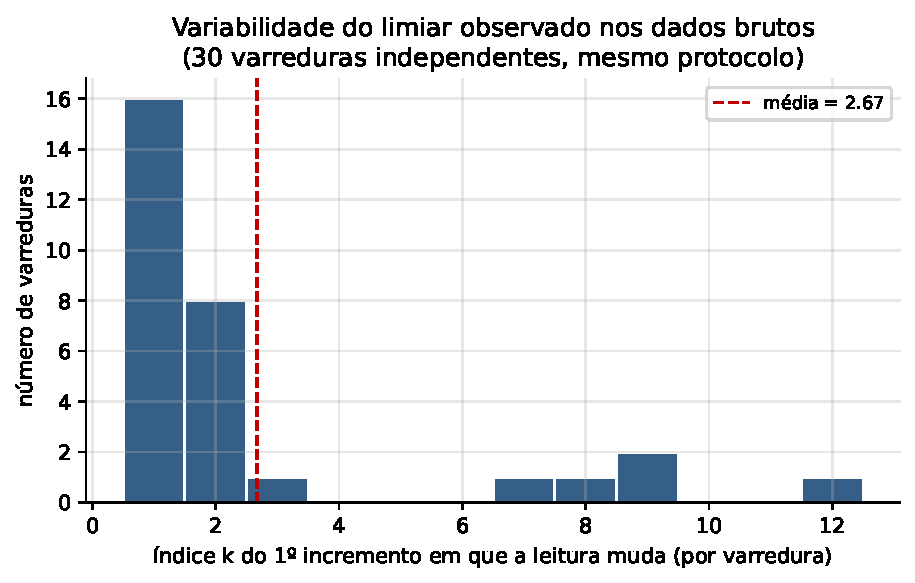
\includegraphics[width=0.68\textwidth]{figs/primeira_transicao_histograma.pdf}
\caption{Variabilidade do limiar observado diretamente nos dados brutos: índice do incremento em
que a leitura muda pela primeira vez, em cada uma das $30$ varreduras independentes. A dispersão
em torno da média é o mesmo fenômeno estatístico caracterizado analiticamente no Ensaio~L3
de~\cite{limiarv1}.}
\label{fig:histograma}
\end{figure}

\begin{caixa}[title={Um detalhe metrológico visível já no ponto de repouso}]
Como o ponto de repouso foi definido exatamente sobre uma transição de código --- a mesma
convenção de \textbf{pior caso} adotada desde o Ensaio~L2 de~\cite{limiarv1} ---, a leitura no
próprio repouso ($k=0$) não é perfeitamente estável: em cerca de metade das $30$ varreduras, uma
amostra de ruído negativa já é suficiente para que a leitura apareça um código abaixo do valor
``ideal'' de repouso, antes mesmo de qualquer incremento ser aplicado. Isso não é um defeito do
dataset --- é o próprio mecanismo de falso alarme discutido no Ensaio~L3 de~\cite{limiarv1}
(Seção~5.2 daquele relatório), agora presente nos dados como um fenômeno a ser identificado pela
análise, não como algo já filtrado pela equipe.
\end{caixa}

% ===========================================================================
\section{Conformidade com as duas exigências obrigatórias da orientação}
\label{sec:conformidade}

\begin{enumerate}[leftmargin=1.6em]
\item \textbf{Ruído de medição incluído deliberadamente.} Cada amostra de
      \texttt{y\_instrumento} passa por uma realização independente de ruído gaussiano antes da
      quantização --- a característica não aparece de forma determinística em nenhum ponto do
      arquivo.
\item \textbf{Nenhum pré-processamento.} \texttt{y\_instrumento} é escrito exatamente como
      produzido pelo modelo a cada amostra: nenhuma média, filtragem ou suavização foi aplicada
      pela equipe antes da exportação. As $30$ varreduras independentes estão concatenadas cruas,
      uma após a outra, sem nenhuma agregação entre elas.
\end{enumerate}

% ===========================================================================
\section{Considerações finais}

Este pacote gerou o conjunto de dados brutos exigido pela~\cite{orientacao2026} para a
característica \textbf{Limiar} do Grupo~08, reaproveitando integralmente a função da
característica estática já construída, caracterizada e validada em~\cite{limiarv1} ---
quantização de $12$~bits e ruído do canal de medição de $\delta$ --- e aplicando o protocolo de
pequenos incrementos crescentes exigido para esta característica. As duas exigências
obrigatórias da orientação (ruído deliberado; ausência de pré-processamento) foram atendidas por
construção, e os próprios dados brutos já exibem, sem que nenhum cálculo de limiar tenha sido
revelado, o comportamento estatístico (e não determinístico) do fenômeno caracterizado
analiticamente em~\cite{limiarv1}.

Conforme a observação final da~\cite{orientacao2026}, este pacote trata apenas da etapa de
geração de dados. As perguntas de análise (Seções~3.1 e~3.2) serão elaboradas pelo professor em
cima do arquivo \texttt{Equipe\_08\_Limiar.csv} efetivamente entregue, e distribuídas em etapa
posterior.

% ===========================================================================
\appendix
\section{Reprodutibilidade}
\label{ap:repro}

\begin{center}\small
\begin{tabular}{@{}ll@{}}
\toprule
\textbf{Item} & \textbf{Especificação}\\
\midrule
Linguagem & Python 3\\
Bibliotecas & NumPy~\cite{numpy2020}, Pandas~\cite{mckinney2010}, Matplotlib~\cite{matplotlib2007}\\
Geração do dataset & \texttt{../gerar\_dados\_limiar.py} (semente fixa $20260903$)\\
Figuras deste relatório & \texttt{figuras\_relatorio.py} (lê o CSV já entregue, não gera dados novos)\\
Determinismo & dataset e figuras reprodutíveis \emph{byte a byte} a partir da semente fixa\\
\bottomrule
\end{tabular}
\end{center}

\begin{caixa}[title={Nota de sigilo sobre \texttt{gerar\_dados\_limiar.py}}]
A~\cite{orientacao2026} registra explicitamente: \emph{``não é necessário revelar os parâmetros
numéricos internos da função geradora''}. O script \texttt{gerar\_dados\_limiar.py} contém esses
parâmetros (o quantum do conversor e o desvio-padrão do ruído) e serve apenas como
\textbf{gabarito de reprodutibilidade interno da equipe} --- o mesmo tratamento já dado a
\texttt{monta\_circuito\_limiar.py}/\texttt{roda\_limiar.py} em~\cite{limiarv1} (mantidos no
pacote de projeto da equipe, fora do material entregue). Se este dataset for repassado a
terceiros para o exercício de análise das Seções~3.1/3.2, apenas a pasta \texttt{dados/} deve
acompanhar a entrega --- o script e este relatório detalhado podem ficar restritos ao
repositório de trabalho da equipe.
\end{caixa}

% ===========================================================================

\begin{thebibliography}{99}

\bibitem{orientacao2026}
UFAL -- ECOM060 -- Instrumentação Eletrônica (2026.2).
\emph{Orientação --- Geração de Dados: Características Estáticas (Seção 3.3)}.
Documento distribuído pelo professor responsável, Maceió, 2026.

\bibitem{limiarv1}
SILVA JUNNIOR, C. M.; PEREIRA, L. L. B.; SANTOS, W. T. O.
\emph{Limiar --- Caracterização do Limiar de Detecção do Sistema Instrumentado: Gerador
Síncrono (Swing Equation), v1}. ECOM060, Universidade Federal de Alagoas, Maceió, 2026.
(Relatório principal, arquivo \texttt{ECOM060\_Relatorio\_Limiar\_Grupo08.pdf}, na raiz deste
repositório.)

\bibitem{vim2012}
JCGM 200:2012.
\emph{International Vocabulary of Metrology --- Basic and General Concepts and Associated Terms
(VIM)}. 3.~ed. Sèvres: BIPM/JCGM, 2012.
(Item~4.16 --- \emph{discrimination threshold}, limiar de discriminação.)

\bibitem{aguirre2015}
AGUIRRE, L. A.
\emph{Fundamentos de Instrumentação}. São Paulo: Pearson Education do Brasil, 2015.
(Seção~3.3 --- características estáticas de instrumentos de medição.)

\bibitem{typhoon}
TYPHOON HIL, INC.
\emph{Typhoon HIL Documentation --- Schematic Editor and Solver}.
Disponível em: \url{https://www.typhoon-hil.com/documentation/}.

\bibitem{numpy2020}
HARRIS, C. R.\ \emph{et al.}
Array programming with NumPy. \emph{Nature}, v.~585, p.~357--362, 2020.

\bibitem{mckinney2010}
McKINNEY, W.
Data structures for statistical computing in Python.
\emph{Proceedings of the 9th Python in Science Conference (SciPy)}, p.~56--61, 2010.

\bibitem{matplotlib2007}
HUNTER, J. D.
Matplotlib: A 2D graphics environment.
\emph{Computing in Science \& Engineering}, v.~9, n.~3, p.~90--95, 2007.

\end{thebibliography}

